%%%%%%%%%%%%%%%%%%%%%%%%%%%%%%%%%%%%%%%%%
% Stylish Article
% LaTeX Template
% Version 2.1 (1/10/15)
%
% This template has been downloaded from:
% http://www.LaTeXTemplates.com
%
% Original author:
% Mathias Legrand (legrand.mathias@gmail.com) 
% With extensive modifications by:
% Vel (vel@latextemplates.com)
%
% License:
% CC BY-NC-SA 3.0 (http://creativecommons.org/licenses/by-nc-sa/3.0/)
%
%%%%%%%%%%%%%%%%%%%%%%%%%%%%%%%%%%%%%%%%%

%----------------------------------------------------------------------------------------
%	PACKAGES AND OTHER DOCUMENT CONFIGURATIONS
%----------------------------------------------------------------------------------------
\documentclass[10pt]{SelfArx} % Document font size and equations flushed left

%fleqn,
\usepackage[T1]{fontenc}
\usepackage{newtxmath,newtxtext}

\usepackage{textcomp}
\usepackage{gensymb}

\usepackage{amsmath, amsfonts}

\usepackage{titlesec}
%\titlespacing*{\section}{-0.5pt}{0.5\baselineskip}{\baselineskip}
%\usepackage[english]{babel} % Specify a different language here - english by default

%----------------------------------------------------------------------------------------
%	COLUMNS
%----------------------------------------------------------------------------------------

\setlength{\columnsep}{0.55cm} % Distance between the two columns of text
\setlength{\fboxrule}{0.75pt} % Width of the border around the abstract

%----------------------------------------------------------------------------------------
%	COLORS
%----------------------------------------------------------------------------------------

\definecolor{color1}{RGB}{0,0,90} % Color of the article title and sections
\definecolor{color2}{RGB}{0,20,20} % Color of the boxes behind the abstract and headings

%	HYPERLINKS
%----------------------------------------------------------------------------------------

\usepackage{hyperref} % Required for hyperlinks
\hypersetup{hidelinks,colorlinks,breaklinks=true,urlcolor=color2,citecolor=color1,linkcolor=color1,bookmarksopen=false,pdftitle={Title},pdfauthor={Author}}

%----------------------------------------------------------------------------------------
%	ARTICLE INFORMATION
%----------------------------------------------------------------------------------------

\JournalInfo{Tanzanian Ministry of Water} % Journal information
\Archive{October 28, 2016} % Additional notes (e.g. copyright, DOI, review/research article)

\PaperTitle{Predicting Water Well Functionality} % Article title


\Authors{Alexis Rouge Carrassat (amr439), Anthony Niznik (an533),  Fan Liu (fl379)} % Authors

\Keywords{} % Keywords - if you don't want any simply remove all the text between the curly brackets
\newcommand{\keywordname}{Keywords} % Defines the keywords heading name

%----------------------------------------------------------------------------------------
%	ABSTRACT
%----------------------------------------------------------------------------------------

\Abstract{The country of Tanzania is currently facing a water supply challenge. Water wells are not being fixed quickly, leading to thousands of people not having access to a clean water supply. The Tanzanian Ministry of Water is trying to predict whether water wells are functional, functional - in need of repair, or not functional so that workers are allocated to fixing water wells rather than checking the status of wells. The Ministry has reached out to us to create a model that is able to predict which water wells are functional and which ones need to be fixed. }

%----------------------------------------------------------------------------------------

\newlength\tindent
\setlength{\tindent}{\parindent}
\setlength{\parindent}{0pt}
\renewcommand{\indent}{\hspace*{\tindent}}

\begin{document}



\flushbottom % Makes all text pages the same height

\noindent \maketitle % Print the title and abstract box  


\tableofcontents % Print the contents section

\thispagestyle{empty} % Removes page numbering from the first page

%----------------------------------------------------------------------------------------
%	ARTICLE CONTENTS
%----------------------------------------------------------------------------------------

\section{Exploratory Data Analysis} % The \section*{} command stops section numbering
\subsection{Data Characteristics}

The data set comprises of a variable matrix with 39 features and 59,400 rows of water wells. The output we wish to predict is whether a water well is functional, non-functional, or functional needs repair (Ordinal Values). There are 9 continuous variables, 26 categorical variables, 2 binary variables, 2 variables with all of the same values, and 1 date column. Some of the more interesting continuous variables include longitude and latitude, altitude of well (GPS height column), and construction year of the well. Some of the categorical variables include Region (like a U.S. State) and installer. 
\\[-1.5\baselineskip]
\break

There were plenty of missing values and questionable zero values in columns. We had 3056 missing values in permit column, 3636 missing in installer, and 3622 missing in funder. Incorrect zero values occurred in the longitude column 1812 times (Longitude Range: 29$^\circ$ E to 41$^\circ$ E) and 18897 times in the construction year column (all other year in 2000s). Our approach to solve these issues will come addressed further in the data cleaning section. To get a sense of where all these water wells are located, we plotted the water wells on a geographical map with blue indicating the well is functioning, and red indicating not functioning (see figure 1).

\setlength{\abovecaptionskip}{15pt plus 3pt minus 2pt}


\setlength{\belowcaptionskip}{-13pt}
\begin{figure}[ht]\centering
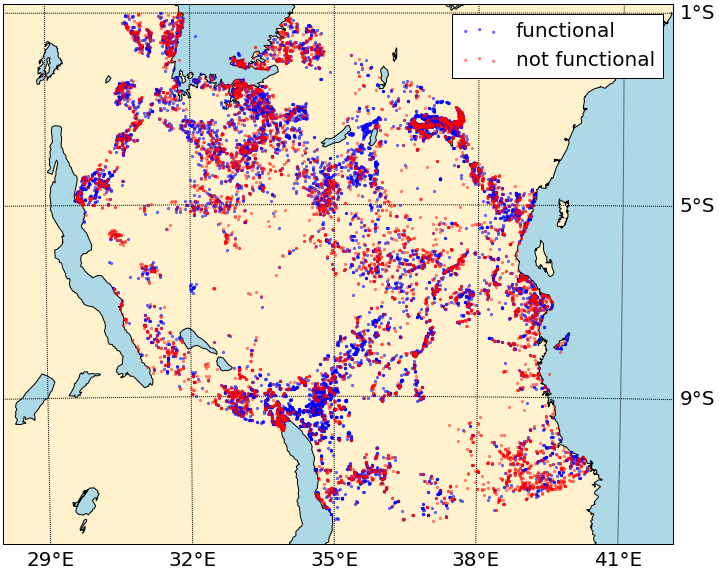
\includegraphics[width=\linewidth]{location.png}
\caption{Locations of Wells in Tanzania}
\label{fig:map}
\end{figure}


\subsection{Data Visualization}

We first used histograms to visualize which variables could separate well functionality most distinctly. We found that whether a water well had a permit (legally authorized to exist) or not greatly affected the classification of the well. If a water well has a permit, it is much more likely to be functional than if it does not have a permit (see figure 2 where a random sample of the data is plotted). This makes permit a strong predicter of functionality of well for our model.
\\[-1.5\baselineskip]
\break

\setlength{\belowcaptionskip}{10pt}
\begin{figure}[ht]\centering
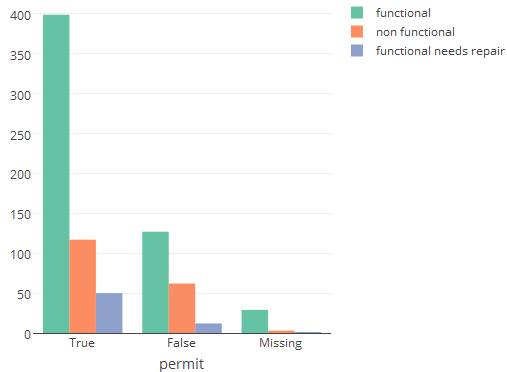
\includegraphics[width=\linewidth]{permit.png}
\caption{Number of Wells Based on Permit}
\label{fig:permit}
\end{figure}

Another question that came up was how the variability in continuous variables could be different depending on the classifications. We considered the variable called GPS Height that gives the height of the water well relative to sea level in meters. We created a boxplot that displays the spread of the GPS Height for functional needs repair, non-functional, and functional wells (see figure 3). We see that the median GPS height of non-functional wells is significantly lower than the median of both functional and functional needs repair wells. This implies that non-functional wells tend to have a lower GPS height than the other wells.
\break

\setlength{\belowcaptionskip}{-15pt}
\begin{figure}[ht]\centering
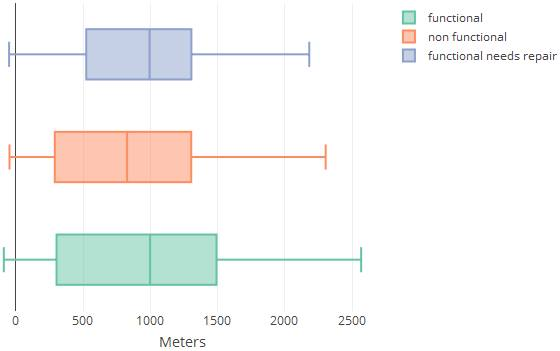
\includegraphics[width=\linewidth]{boxplot2.png}
\caption{Well Classification Based on GPS Height}
\label{fig:GPS}
\end{figure}

While going through the different features, we quickly realized that longitude and latitude both were important features for classification. Though we plotted the water wells onto the map of Tanzania, we wanted to get a better idea of where most of the functional wells may be located. We created a plot of longitude vs latitude this time to see if we can get a better sense of where the functional wells were. We were able to pinpoint a rectangular area  in the center of Tanzania (shaded in blue) where over 70\% of wells are functional (see figure 4 where a random sample of the data is plotted).
\\[-1.5\baselineskip]
\break

\setlength{\belowcaptionskip}{0pt}
\begin{figure}[ht]\centering
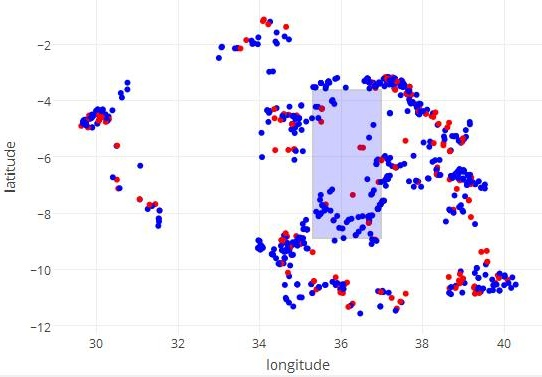
\includegraphics[width=\linewidth]{map_color2.jpg}
\caption{Longitude Vs Latitude of Wells; Functional Wells (Blue), Non-Functional Wells (Red)}
\label{fig:map2}
\end{figure}

After this discovery, we considered the 21 regions in Tanzania and the percent of non-functional water wells in each region. When we created a bar plot that ordered the regions from lowest longitude to highest longitude (West to East), we found that the regions in the center of Tanzania (Iringa, Akusha, and Manyara) had some of the lowest percentages of non-functional wells (see figure 5). This means that we can explore these regions further to see which characteristics they may have that leads to a high percentage of functional wells. 

\setlength{\belowcaptionskip}{-15pt}
\begin{figure}[ht]\centering
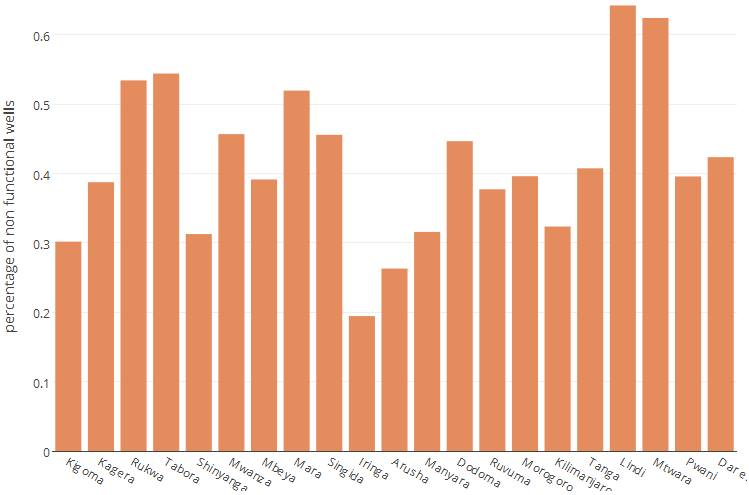
\includegraphics[width=\linewidth]{barplot2.png}
\caption{Barplot of Percent of Non-Functional Wells Based on Regions that are Ordered By Longitude (Left to Right)}
\label{fig:barplot}
\end{figure}

\subsection{Cleaning the Data}

We immediately left out of our model any columns that were nearly duplicates of each other (more than 95\% of same row values and measuring same thing). Then, we changed the column that had calendar date of well status check (day, month, year) to just the number of days from the current date to the earliest date of water well status check. So, if the earliest date any well was checked is 10/14/2002, then a well checked on 12/03/2013 would have 4069 as its value. We also transformed the installer column (which company installed the well). Since there are 2113 unique installer values and the majority of rows belonged to the top two installers (outliers compared to the rest of the data), we simply created three new binary variables (one for the installer with the most wells, one for the installer with the second most wells, all other installers placed in a "other" column, and a column for missing values discussed in the next paragraph.)
\\[-1.5\baselineskip]
\\[0\baselineskip]
\break
For the categorical variables, we used one-hot encoding to change a variable of one column and d distinct values to d binary variable columns. This increased the number of columns of our model from 28 to 220 columns. If values were missing from a particular column, we created a new binary variable that takes one if a value is missing and zero otherwise. In this way, we could retain some information, even for missing values and not have to delete an entire row just for 1 missing value.  For logistic regression, we standardized continuous variables such as longitude and latitude of water well since regularized least squares is not scaling invariant.
\\[-1.5\baselineskip]
\\[0\baselineskip]
\break
We noticed for some variables such as population and GPS height that the distribution of classification (functional, not functional) is very different for the wells with zeros and the wells with a value higher than zero in our data visualization (see figure 3). Due to this, we added a binary variable column that indicates for population whether it is zero or greater than zero since zero appears very often (33\%). Additionally, the variance of population and GPS height in well is very high so we took the natural log of these variables to make sure that values that are greater than zero but small will still have a significant impact on the model.

\section{Model Selection}

\subsection{Logistic Regression}

For our initial model, we chose to use logistic regression model (denoted by $h(x)$) because the water well problem is a classification problem. We first split the data into 60\% training set, 20\% validation set, and 20\% testing set. We used the validation set to calculate the $\lambda$ that minimizes the percent of misclassifications. The objective function of logistic regression is defined as the following: 

\begin{equation}
 h(x) = log(1+e^{(-yw^Tx)}) + \lambda||w||_1
\end{equation}

Since logistic regression is a binary logistic model (1 if water well is a certain classification and 0 otherwise), we could not simply use one regression to perform the analysis. Instead, we created 3 different logistic regression models for each class i (one for each classification of functional, non-functional, functional - needs repair). We then used that fact the logistic regression returns the probability that a water well is a certain classifcation to just simply take the maximum probability of the three models in order to classify the well (see equation 2).

\begin{equation}
 y= \underset{i}{\mathrm{argmax}}\, h_i(x) 
\end{equation}

\subsection{Random Forest}

Another model we considered is random forest. The way random forest works is that it takes a collection of random samples from the training set while maintaining the underling distribution. Then, it creates groups of decisions trees (x) where each tree is assigned a certain number of features at random. Each decision tree is split on each feature based on maximizing the amount of information we can gain from each split (create the greatest reduction in entropy). When it comes time to predict, a majority vote is taken from each group of decision trees to classify each water well (see figure 6).  
\\[-1.5\baselineskip]
\break

\setlength{\belowcaptionskip}{-10pt}
\begin{figure}[ht]\centering
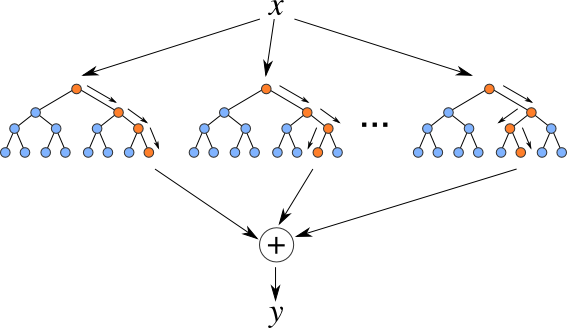
\includegraphics[width=6cm, height=3.8cm]{rf.png}
\caption{Random Forest Example}
\label{fig:rf}
\end{figure}

For our random forest model,  we used 30 trees in our forest. We allowed trees to grow to a maximum depth of 20 and assigned trees to randomly pick the square root of the total number of features to split upon. The number of features to split upon and the maximum depth are parameters that we will fine tune later in the project. Random forest prevents underfitting since trees are randomly assigned to a subset of features to split on which helps to account for all the different characteristics water wells may have (flexible). Also, random forest is not prone to overfitting since the majority vote of a group of trees prevents overfit trees from weighing heavily on the classification. 

\section{Results}

To test the effectiveness of both models, we calculated accuracy as the percentage of correctly classified water wells in our testing set by the models. We found that logistic regression was able to classify with an accuracy of about 73\%. On the other hand, random forest was able to classify with an astonishing 80\% accuracy. An indication that the accuracy of the test data is low for logistic regression may lie in the fact that the training error for logistic regression is also low (about 74\% also) which implies that logistic regression has a relatively high bias.

\section{Next Steps}

To improve our model, we will look to transform some of our variables in order to capture information better than simply including data in its raw state. For example, we can add a binary column that indicates whether the well was checked in the dry season or the rainy season. This can show trends of how weather seasonality may relate to the probability of a water well being functional. Our goal is to be able to classify water wells with the most accuracy and even to classify better than the current best model for this problem (classifies with 82\% accuracy). Another route worth considering is to help the Tanzanian Ministry of Water learn about which features lead to the highest likelihood of a water well functioning properly. This could help the Ministry to know how to build new water wells so that they are more likely to work.

\end{document}
